%BAB_2 LAPORAN KP
\chapter{LANDASAN TEORI}

\section{Gambaran Umum Robot Lengan}

Robot adalah adalah sebuah alat yang terdiri dari gabungan mekanik dan elektronik yang dapat melakukan tugas fisik, baik menggunakan pengawasan, kendali manusia maupun secara otomatis. Robot dapat melakukan suatu tugas secara berulang tanpa merasa lelah sehingga robot banyak digunakan dalam dunia industri khususnya pada bidang produksi. Salah satu jenis robot yang sering digunakan dalam bidang produksi adalah sistem lengan robot.

Robot lengan adalah robot yang memiliki bentuk fisik seperti halnya lengan pada manusia dan memiliki derajat kebebasan (\emph{Degre of Freedom}) tertentu bergantung pada jumlah sendi yang digunakan. Robot lengan pada bidang industri biasa digunakan sebagai aktuator untuk mengambil dan meletakkan suatu objek secara terus menerus.
	

Pada umumnya struktur robot lengan terdiri dari beberapa bagian.  Bagian utama dari robot lengan adalah struktur mekanik ({\textit{Manipulator}}) yang merupakan susunan kerangka yang tidak dapat digerakkan (\emph{Rigid}) dan lengan (\emph{Link}) yang satu sama lain terhubung oleh sendi (\emph {joint}). Dengan adanya \emph{joint} yang menghubungkan dua \emph{link} menjadi satu kesatuan sehingga \emph{joint} membentuk satu derajat kebebasan. Jika diibaratkan dengan tubuh manusia, \emph{link} adalah tulang sedangkan \emph{joint} adalah sendi-sendinya. \emph{Joint} memiliki dua pergerakan, yaitu pergerakan \emph{revolute joint} (gerak berputar) dan \emph{prismatic joint} (gerak bergeser). Gambar \ref{pic.jenisjoint} merupakan jenis-jenis dari \textit{joint}.

	\begin{figure}[H]
	\centering
	\includegraphics[width=11cm]{gambar/joint.png}
	\caption{Jenis-Jenis \textit{Joint}}
	\label{pic.jenisjoint}
\end{figure}


\subsection{\emph{Degress of Freedom }}
\emph{Degress of Freedom} (DOF) merupakan sebuah konfigurasi yang dapat meminimalkan spesifikasi dengan menggunakan parameter yang dapat menyatakan posisi suatu sistem pada setiap saat. Umumnya robot lengan mempunyai paling sedikit enam independen derajat kebebasan, tiga derajat kebebasan untuk translasi dan tiga derajat kebebasan untuk rotasi. Robot lengan paling tidak memiliki tiga derajat kebebasan untuk dapat memiliki \emph{workspace} yang cukup. \emph{Workspace} dari sebuah robot lengan merupakan total volume yang dapat dijangkau oleh \emph{end-effector} dari pergerakan semua \emph{joint}-nya dari titik minimum hingga maksimum. 

\subsection{Konfigurasi Robot Lengan}
Pada dasarnya berbagai jenis dari robot lengan dapat dibedakan dari konfigurasinya. Konfigurasi robot lengan merupakan perpaduan antara pergerakan \emph{joint} yang dimiliki oleh robot lengan. Konfigurasi ini memiliki tipe yang berbeda-beda sehingga \emph {workspace} yang dimiliki pada tiap robot lengan pasti berbeda.

\subsubsection{Konfigurasi \emph{Articulated} (\emph{Revolute - Revolute - Revolute)}} 
\emph{Articulated} manipulator ini pada dasarnya mempunyai jenis \emph{revolute joint} pada ketiga \emph{joint} robot lengan (\emph {base, shoulder, elbow}). Dengan konfigurasi ini, robot lengan dengan konfigurasi \textit{Articulated} dapat memiliki variasi DOF yang banyak. DOF yang dapat dihasilkan dengan robot lengan dengan konfigurasi seperti ini adalah tiga DOF hingga sampai dengan enam DOF tergantung dari kebutuhan dan fungsi yang akan dilakukan oleh robot lengan. Konfigurasi dari \textit{joint revolute} ini menjadikan robot lengan jenis ini mempunyai kebebasan yang besar dari pergerakannya dalam ruang yang kecil sehingga menjadikan jenis konfigurasi \textit{Articulated} manipulator ini banyak dipakai dan memiki desain yang populer. Gambar \ref{pic.articulated} merupakan konfigurasi dari \textit{Articulated}.
	\begin{figure}[H]
	\centering
	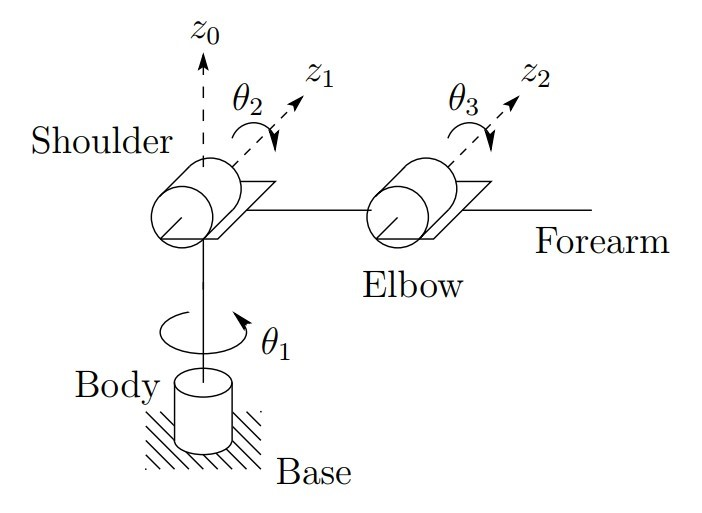
\includegraphics[width=8cm]{gambar/articulated.jpg}
	\caption{Struktur dari Konfigurasi  \textit{Articulated}}
	\label{pic.articulated}
\end{figure}
\subsubsection{Konfigurasi \textit{Spherical} (\textit{Revolute – Revolute – Prismatic})} 

Konfigurasi \textit{Spherical} merupakan konfigurasi yang mempunyai dua buah \textit{joint revolute} dan satu buah \textit{joint prismatic}. \textit{Joint prismatic} berada ini \textit{joint} ketiga atau pada bagian \textit{elbow}. Sementara dua \textit{joint} lainnya berada di \textit{shoulder} dan \textit{wrist}. Gambar \ref{pic.spherical} merupakan struktur dari konfigurasi \textit{Spherical}.
	\begin{figure}[H]
	\centering
	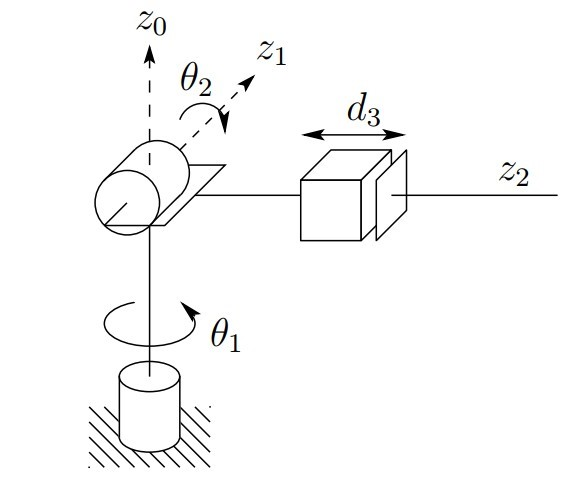
\includegraphics[width=8cm]{gambar/spherical.jpg}
	\caption{Struktur dari Konfigurasi \textit{Sperical}}
	\label{pic.spherical}
\end{figure}


\subsubsection{Konfigurasi SCARA (\textit{Revolute – Revolute – Prismatic}) } 

Konfigurasi \textit{Selective Compliant Articulated Robot for Assembly} (SCARA) merupakan konfigurasi yang mempunyai dua buah \textit{joint revolute} dan satu buah \textit{joint prismatic} sama seperti konfigurasi \textit{Spherical}. Meskipun SCARA memiliki struktur \textit{joint revolute – revolute – prismatic} (RRP) sama seperti konfigurasi yang dimiliki \textit{Spherical}, struktur ini sedikit berbeda dengan konfigurasi \textit{Spherical} dari tampilannya maupun dari jarak \textit{workspace} nya. Tidak seperti konfigurasi \textit{Spherical}, dimana $z_{0}$ tegak lurus terhadap $l$, dan $z_{1}$ tegak lurus dengan $z_{2}$, konfigurasi SCARA memiliki struktur $z_{0}, z_{1}, dan z_{2}$ yang paralel. Gambar \ref{pic.scara} merupakan struktur dan konfigurasi dari SCARA.
	\begin{figure}[H]
	\centering
	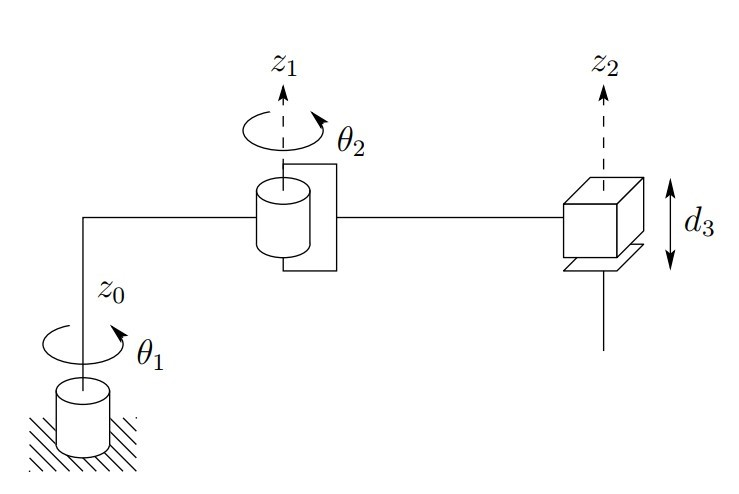
\includegraphics[width=8cm]{gambar/scara.jpg}
	\caption{Struktur dari Konfigurasi SCARA}
	\label{pic.scara}
\end{figure}

\subsubsection{Konfigurasi \textit{Cylindrical} (\textit{Revolute – Prismatic – Prismatic}) } 

Konfigurasi \textit{Cylindrical} merupakan konfigurasi yang mempunyai satu buah \textit{joint revolute} dan dua buah \textit{joint prismatic}. \textit{Joint revolute} menghasilkan pergerakan rotasi di \textit{base}, sementara \textit{joint prismatic} berada di bagian \textit{shoulder} dan \textit{elbow}. Gambar \ref{pic.cylindrical} merupakan struktur dari konfigurasi \textit{Cylindrical.}
\begin{figure}[H]
	\centering
	\includegraphics[width=5cm]{gambar/cylindrical.jpg}
	\caption{Struktur dari Konfigurasi \textit{Cylindrical}}
	\label{pic.cylindrical}
\end{figure}
\subsubsection{Konfigurasi \textit{Cartesian} (\textit{Prismatic – Prismatic – Prismatic})  } 

Konfigurasi \textit{Cartesian} mempunyai tiga buah \textit{joint prismatic}. Variabel \textit{joint} dari konfigurasi \textit{prismatic} adalah koordinat \textit{Cartesian} dari \textit{end-effector} dengan memperhatikan letak \textit{base} dari robot lengan. Kinematika dari jenis konfigurasi ini adalah yang paling sederhana dari semua konfigurasi robot lengan. Konfigurasi \textit{Cartesian} sangat berguna untuk penyusunan suatu barang di bidang datar seperti mesin laser, kargo atau memindahkan barang. Gambar \ref{pic.cartesian} merupakan struktur dari konfigurasi \textit{Cartesian}.

	\begin{figure}[H]
	\centering
	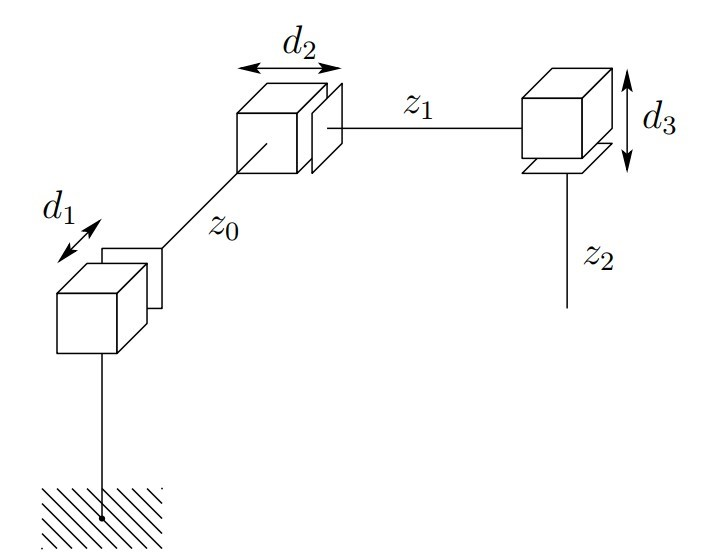
\includegraphics[width=6cm]{gambar/cartesian.jpg}
	\caption{Struktur dari Konfigurasi \textit{Cartesian}}
	\label{pic.cartesian}
\end{figure}

\subsection{ \textit{Wrist} dan \textit{End-effector} }

\textit{Wrist} atau pergelangan tangan merupakan \textit{joint} diantara lengan dan \textit{end-effector}. \textit{Joint wrist} ini pada umumnya terdapat \textit{joint revolute} . Hal ini umum digunakan pada desain manipulator lengan dengan konfigurasi \textit{Spherical}. Konfigurasi \textit{Spherical} mempunyai \textit{joint revolute} yang saling berpotongan diantara ketiganya, maksudnya setiap \textit{joint} berputar sesuai koordinat $x, y $ dan $z$. Rotasi atau perputaran dengan \textit{axis} sumbu $x$ adalah \textit{roll}, perputaran dengan \textit{axis} sumbu $y$ adalah \textit{pitch} dan perputaran dengan \textit{axis} sumbu $z$ adalah \textit{yaw}. Gambar \ref{pic.sphericalwirst} merupakan struktur dari konfigurasi \textit{Spherical Wirst.}
	\begin{figure}[H]
	\centering
	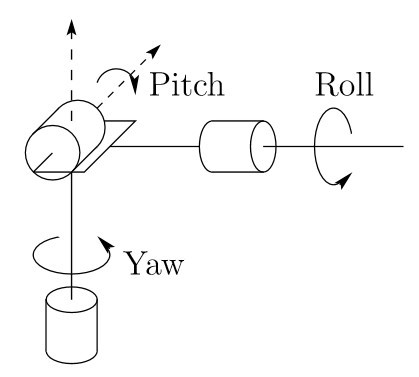
\includegraphics[width=5cm]{gambar/wirst.jpg}
	\caption{Struktur dari \textit{Joint Spherical Wrist}}
	\label{pic.sphericalwirst}
\end{figure}


\textit{End-effector} merupakan perangkat atau alat yang terhubung dengan ujung lengan robot. \textit{End-effector} adalah bagian robot yang berhubungan langsung dengan objek. Struktur, pergerakan, material dari \textit{end-effector} bergantung pada tugas yang akan dilakukan robot tersebut. Gambar \ref{pic.endeffector} merupakan bentuk dari \textit{end-effector.}
	\begin{figure}[H]
	\centering
	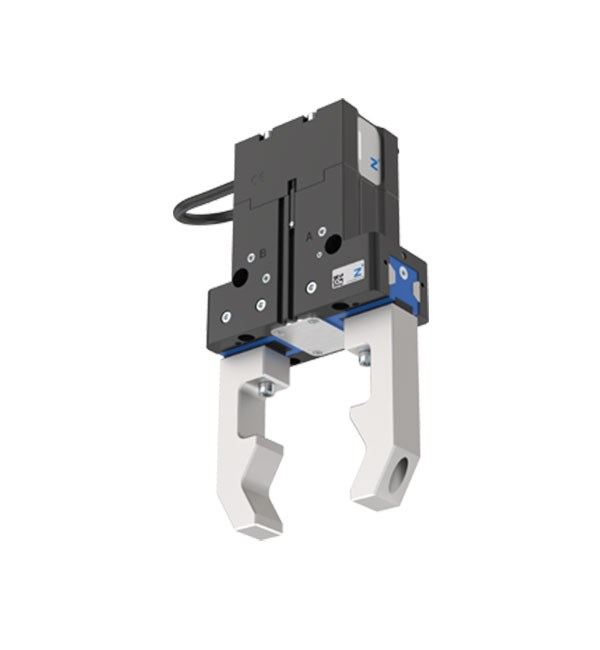
\includegraphics[width=6cm]{gambar/end_effector.jpg}
	\caption{Struktur \textit{End-Effector}}
	\label{pic.endeffector}
	\end{figure}


\section{Kinematika}
Kinematika merupakan pembelajaran pergerakan tubuh robot tanpa memperhitungkan gaya, torsi maupun momen tertentu yang menyebabkan pergerakan. Terdapat berbagai jenis pergerakan dari kinematika yang tergantung dari tujuan dari setiap robot. Kinematika yang dijelaskan pada penelitian ini adalah kinematika yang khusus mempelajari dan menganalisa pergerakan robot lengan.  

Pada kinematika robot terdapat dua buah pembahasan kinematika. Pembahasan pertama adalah kinematika maju yang merupakan proses menghitung orientasi dan posisi dari\textit{ end-effector} berdasarkan nilai sudut pada masing-masing \textit{joint}.  Sedangkan kinematika balik sebaliknya dari kinematika maju, diberikan posisi \textit{end-effector} dimana dicari  besaran sudut yang harus diubah untuk tiap \textit{joint} dalam mencapai posisi \textit{end-effector} tersebut. Gambar \ref{pic.diagram.kinematika} merupakan diagram blok sederhana dari pemodelan kinematika.
	\begin{figure}[H]
	\centering
	\includegraphics[width=12cm]{gambar/kinematika_diagram.png}
	\caption{Blok Diagram Kinematika}
	\label{pic.diagram.kinematika}
\end{figure}

\subsection{Kinematika Maju}
Kinematika maju atau biasa disebut \textit{forward kinematics} merupakan kinematika untuk mendapatkan hasil akhir berupa koordinat posisi ($x, y, z$) dengan diketahuinya variabel sudut pada setiap \textit{joint} dari lengan robot.  Variabel sudut tersebut kemudian dilakukan perhitungan satu sama lain hingga pada akhirnya akan mendapatkan koordinat $x$, koordinat $y$, dan koordinat $z$. Gambar \ref{pic.kinematikamaju} merupakan proses dari kinematika maju.
	\begin{figure}[H]
	\centering
	
\includegraphics[width=12cm]{gambar/Kinematika_maju.png}
	\caption{Kinematika Maju}
	\label{pic.kinematikamaju}
\end{figure}


\subsection{Kinematika Balik}
Kinematika balik (\textit{inverse kinematics}) digunakan untuk mencari variabel sudut (\textit{joint}) robot dalam menentukan posisi dan orientasi dari \textit{end-effector}. Dalam menentukan koordinat \textit{end-effector}, kinematika balik mengacu pada penggunaan persamaan kinematika robot untuk menentukan parameter bersama yang memberikan posisi yang diinginkan pada posisi akhir atau \textit{end-effector}.  Dalam pergerakannya, robot dimodelkan dalam bentuk persamaan kinematika. Persamaan ini menentukan konfigurasi robot dalam hal parameter untuk setiap aktuator. Kinematika maju menggunakan parameter untuk menghitung konfigurasi robot, dan kinematika balik membalikkan perhitungan ini untuk menentukan parameter bersama dalam mencapai konfigurasi yang diinginkan. 

Secara garis besar metode kinematika balik mencari nilai-nilai parameter yang harus diberikan kepada setiap aktuator untuk mencapai tujuan akhir. Untuk mendapatkan nilai-nilai parameter tersebut, robot harus mengetahui terlebih dahulu manipulator yang dimilikinya, baik ukuran maupun jumlah aktuator serta derajat kebebasan yang ada. Kemudian robot harus ditanamkan rumus-rumus yang didapat dari berbagai model perhitungan, baik dari segi analisa grafik langsung maupun menggunakan metode-metode dari berbagai penelitian. Gambar \ref{pic.kinematikabalik} merupakan proses dari kinematika balik.

	\begin{figure}[H]
	\centering
	\includegraphics[width=10cm]{gambar/kinematika_balik.png}
	\caption{Kinematika Balik}
	\label{pic.kinematikabalik}
\end{figure}

\section{Motor DC}
Motor DC adalah motor listrik yang memerlukan suplai tegangan arus searah pada kumparan medan untuk diubah menjadi energi gerak mekanik. Motor DC mempunyai dua bagian utama, yaitu stator dan rotor. Stator merupakan bagian yang tidak berputar dan rotor merupakan bagian yang berputar dan merupakan kumparan jangkar. Motor DC menghasilkan jumlah putaran dalam setiap satuan waktu yang biasanya dihitung setiap satuan menit (\textit{rotations per minute}) dan dapat diatur arah putaranya searah jarum jam (\textit{clock wise}) atau berkebalikan dengan arah jarum jam (\textit{counter clock wise}) bergantung dengan kutub atau polaritas dari catu daya yang diberikan pada motor DC. Gambar \ref{[pic.motordc} merupakan bentuk fisik dari motor DC.
	\begin{figure}[H]
	\centering
	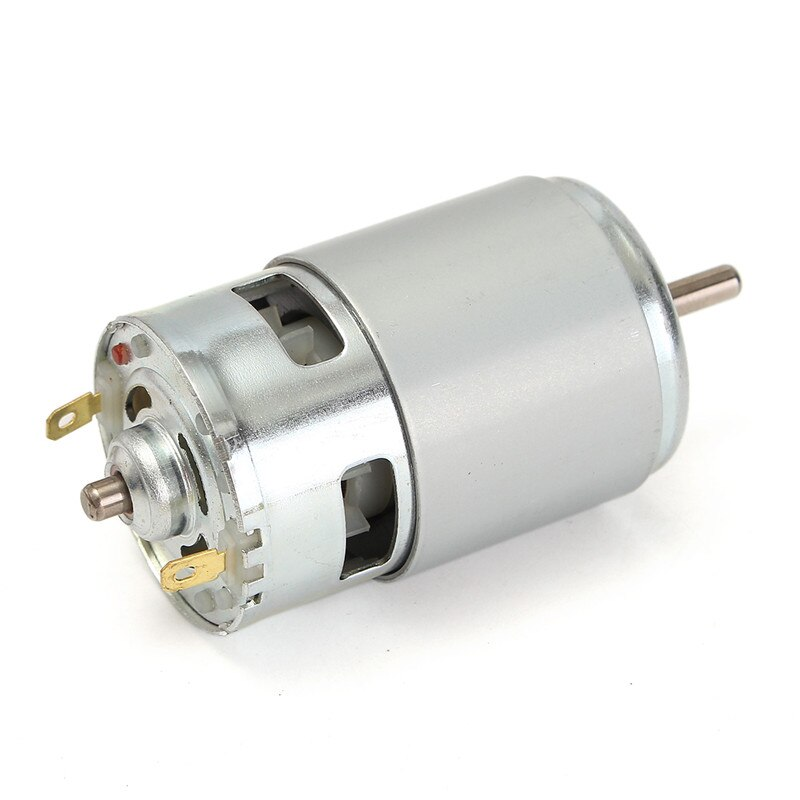
\includegraphics[width=4cm]{gambar/motorDC.jpeg}
	\caption{Bentuk Fisik Motor DC}
	\label{pic.motordc}
\end{figure}

Motor DC dapat bergerak karena adanya elektromagnet. Saat kumparan diberi arus listrik, permukaan kumparan yang bersifat utara akan bergerak menghadap ke magnet yang berkutub selatan dan kumparan yang bersifat selatan akan bergerak menghadap ke utara magnet. Pada saat ini, kerena kedua kutub saling menyebabkan pergerakan kumparan berhenti. Untuk menggerakannya lagi tepat pada saat kutub kumparan berhadapan dengan kutub magnet, arah arus pada kumparan dibalik. Dengan demikian, kutub utara kumparan akan berubah menjadi kutub selatan dan kutub selatannya akan berubah menjadi kutub utara.  

Pada saat perubahan kutub tersebut terjadi, kutub selatan kumparan akan berhadapan dengan kutub selatan magnet dan kutub utara kumparan akan berhadapan dengan kutub utara magnet. Karena kutubnya sama, maka akan terjadi tolak menolak sehingga kumparan bergerak memutar hingga utara kumparan berhadapan dengan selatan magnet dan selatan kumparan berhadapan dengan utara magnet. Siklus ini akan berulang-ulang hingga arus listrik pada kumparan diputuskan. Gambar \ref{pic.motordcprinsipkerja} merupakan prinsip kerja dari motor DC.
	\begin{figure}[H]
	\centering
	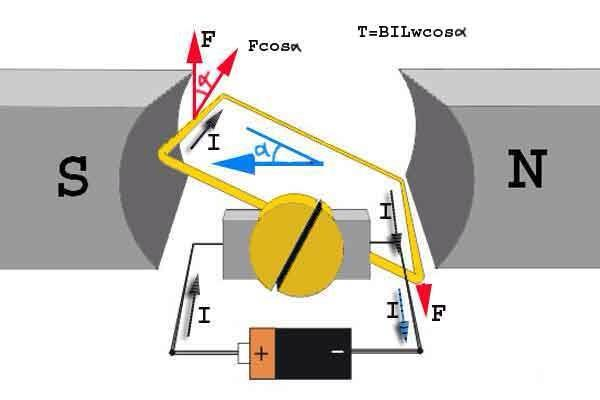
\includegraphics[width=4cm]{gambar/prinsipDC.jpg}
	\caption{Prinsip Kerja Motor DC}
	\label{pic.motordcprinsipkerja}
\end{figure}


\section{Regulator}
Dalam suatu rangkaian elektronika dibutuhkan suatu sumber tegangan yang stabil dan sesuai dengan nilai yang dibutuhkan oleh komponen. Untuk memenuhi kebutuhan tersebut digunakanlah sebuah rangkaian regulator. Rangkaian regulator berfungsi untuk mengatur atau menghasilkan nilai tegangan pada nilai tertentu dari suatu tegangan masukan. Regulator dapat mempertahankan nilai tegangan yang keluar tanpa dipengaruhi besar arus yang dikeluarkannya. Regulator tegangan mempunyai banyak jenisnya, salah satunya adalah regulator \textit{switching}.

Regulator \textit{switching} mengatur besarnya nilai tegangan keluaran dengan mensaklar (ON/OFF) tegangan masukan dengan frekuensi berbeda – beda. Kelebihan dari regulator \textit{switching} adalah mempunyai disipasi daya yang terjadi lebih kecil dibandingkan dengan regulator linear. Sedangkan kekurangannya yaitu tegangan keluaranya akan berbentuk gelombang akibat adanya proses \textit{switching}. Oleh karena itu, regulator jenis ini umumnya membutuhkan induktor, kapasitor, dan dioda untuk memperhalus tegangan keluaran. Regulator \textit{switching} ada dua jenis yaitu regulator \textit{Buck} dan regulator \textit{Boost}. Regulator \textit{Buck} untuk menghasilkan nilai tegangan keluaran yang lebih kecil dari tegangan masukannya. Sedangkan Regulator \textit{Boost} untuk menghasilkan nilai tegangan yang lebih besar dari tegangan masukannya. Salah satu jenis dari regulator \textit{Buck} adalah LM2596 . Gambar \ref{pic.lm2596} merupakan bentuk fisik dari regulator \textit{Buck} LM2596.

	\begin{figure}[H]
	\centering
	\includegraphics[width=7cm]{gambar/lm2596.jpg}
	\caption{Regulator \textit{Buck} LM2596}
	\label{pic.lm2596}
\end{figure}

\section{Arduino Mega 2560}
Arduino Mega 2560  merupakan papan pengembangan dari mikrokontroler yang menggunakan basis Arduino serta menggunakan microchip AT 2560. Arduino  memiliki pin \textit{input} dan \textit{output} dengan jumlah yang cukup banyak, yaitu sejumlah 54 buah pin \textit{input} dan \textit{output} yang 15 diantaranya merupakan pin \textit{Pulse With Modulation} (PWM), 16 diantaranya merupakan pin \textit{analog input}, dan terdapat empat pin yang digunakan sebagai UART (\textit{Serial port hardware}). Arduino ini sudah dilengkapi dengan \textit{oscillator} sebesar 16Mhz, sebuah \textit{port} USB, \textit{power jack} DC, ICSP \textit{header} serta tombol reset. Gambar \ref{pic.arduinomega} merupakan bentuk fisik dari Arduino Mega 2560.
	\begin{figure}[H]
	\centering
	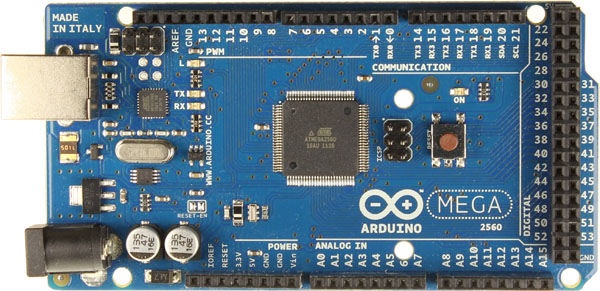
\includegraphics[width=5cm]{gambar/arduino_mega.jpg}
	\caption{Arduino Mega 2560}
	\label{pic.arudinomega}
	\end{figure}

Arduino Mega 2560 memuat semua yang dibutuhkan untuk mendukung kerja dari sebuah mikrokontroler. Arduino Mega 2560 dapat dengan mudah dioperasikan untuk pengaplikasian ke sebuah sistem kerja karena dapat dihubungkan dengan kabel USB sebagai komunikasinya. Untuk dayanya, Arduino Mega 2560 dapat dihidupkan melalui konektor DC yang dipunyainya dengan diberi tegangan DC, atau baterai dengan nilai tegangan sesuai dengan spesifikasi pada Arduino Mega tersebut. Tabel \ref{tbl.arduinomega} merupakan spesifikasi dari Arduino Mega 2560.
\begin{table}[H]
	\centering
	\caption{ Spesifikasi Arduino Mega 2560 }
	\label{tbl.arduinomega}
	\resizebox{14cm}{!}{%
		\begin{tabular}{|l|l|}
		\hline
		Mikrokontroler     & Atmega2560$$\hspace{2cm} 		\\ \hline
		Tegangan operasional     & 5 V$$  				\\ \hline
		Tegangan masukan  & 5-12 V$$  		\\ \hline
		Pin digital I/O       & 54 (15 pin untuk keluaran PWM) $$   \\\hline
		Pin analog masukan     & 16$$ 		\\ \hline
		Arus DC per Pin I/O  & 20 mA $$   				\\ \hline
		Arus DC untuk Pin 3.3 V & 50 mA $$  				\\ \hline
		Memori flash    & 256 KB $$ 		\\ \hline
		Kecepatan clock & 16 MHz $$   				\\ \hline
		Dimensi & 101.52 x 53.3 mm $$  				\\ \hline
		
		\end{tabular}%
}
\end{table}

\section{\textit{Driver} Motor H-\textit{Bridge} EMS 30A}
\textit{Driver} Motor H-\textit{Bridge} EMS 30A berfungsi sebagai pengontrol dari setiap pergerakan dari motor DC. Pergerakan seperti kecepatan, arah putar serta lamanya pergerakan motor DC dapat dikontrol oleh sebuah \textit{Driver} Motor H-\textit{Bridge} EMS 30A.Umunya \textit{driver} motor memiliki beberapa jenis tergantung dari spesifikasi dari motor DC yang digunakan. Salah satu jenis \textit{driver} motor adalah \textit{Driver} Motor  H-\textit{Bridge} EMS 30A. Gambar \ref{pic.drivermotor} merupakan bentuk fisik dari \textit{Driver} Motor H-\textit{Bridge} EMS 30A.

	\begin{figure}[H]
	\centering
	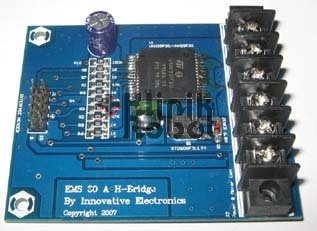
\includegraphics[width=5cm]{gambar/driver_motor.jpg}
	\caption{\textit{Driver} Motor EMS 30A H-\textit{Bridge}}
	\label{pic.drivermotor}
	\end{figure}

\textit{Driver} Motor EMS 30A H-\textit{Bridge} merupakan \textit{driver} motor yang dapat mengoperasikan sebuah Motor DC dengan batasan arus hingga 30 Ampere. Driver ini memiliki 10 buah pin data yang dapat dihubungkan dengan sebuah mikrokontroler. Tabel \ref{tbl.pindrivermotor} merupakan alokasi pin pada \textit{Driver} Motor H-\textit{Bridge} EMS 30A..
% Please add the following required packages to your document preamble:
% \usepackage[normalem]{ulem}
% \useunder{\uline}{\ul}{}
\begin{table}[H]
		\centering
	\caption{ Pin pada \textit{Driver} EMS 30A H-\textit{Bridge} }
	\label{tbl.pindrivermotor}
	\resizebox{14cm}{!}{%
	\begin{tabular}{|c|c|c|l|}
		\hline
		Pin  & Nama & I/O & \multicolumn{1}{c|}{Fungsi}                                                                                                                                                 \\ \hline
		1    & MIN1 & I   & Pin input untuk menentukan output MOUT1                                                                                                                                     \\ \hline
		2    & MIN2 & I   & Pin input untuk menentukan output MOUT2                                                                                                                                     \\ \hline
		3    & MEN1 & I/O & \begin{tabular}[c]{@{}l@{}}Pin enable untuk output MOUT1 \\ diberi logika HIGH untuk mengaktifkan half H-Bridge 1, \\ diberi logika LOW untuk menonaktifkannya\end{tabular} \\ \hline
		4    & MEN2 & I/O & \begin{tabular}[c]{@{}l@{}}Pin enable untuk output MOUT2 \\ diberi logika HIGH untuk mengaktifkan half H-Bridge 2, \\ diberi logika LOW untuk menonaktifkannya\end{tabular} \\ \hline
		5    & MSC  & O   & Output tegangan analog yang berbanding lurus dengan arus beban                                                                                                              \\ \hline
		6    & MPWM & I   & Pin input untuk mengatur kerja modul H-Bridge secara PWM                                                                                                                    \\ \hline
		7,9  & VCC  & -   & Terhubung ke catu daya untuk input (5 Volt)                                                                                                                                 \\ \hline
		8,10 & PGND & 0   & Titik referensi untuk caru daya input                                                                                                                                       \\ \hline
	\end{tabular}}
\end{table}

\section{Processing \textit{Integrated Development Environment} (IDE)}
Processing IDE adalah pemrograman sederhana yang diciptakan untuk pengembangan aplikasi yang berorientasi visual atau pencitraan dengan penekanan pada animasi dan memberi pengguna umpan balik melalui interaksi antarmuka. Para \textit{developer} Processing IDE ini menginginkan sebuah cara untuk "membuat sketsa" gagasan dalam bentuk kode. Karena pemrograman telah berkembang selama beberapa dekade terakhir. Processing IDE telah mulai digunakan untuk pekerjaan tingkat produksi yang lebih maju. Awalnya dibangun sebagai ekstensi khusus \textit{domain} Java yang ditargetkan untuk seniman dan desainer, Processing IDE telah berkembang menjadi alat desain dan prototipe lengkap dan penuh yang digunakan untuk pekerjaan instalasi skala besar, grafis gerak, dan visualisasi data yang rumit. Gambar \ref{pic.processingide} merupakan tampilan pada Processing IDE.
	\begin{figure}[H]
	\centering
	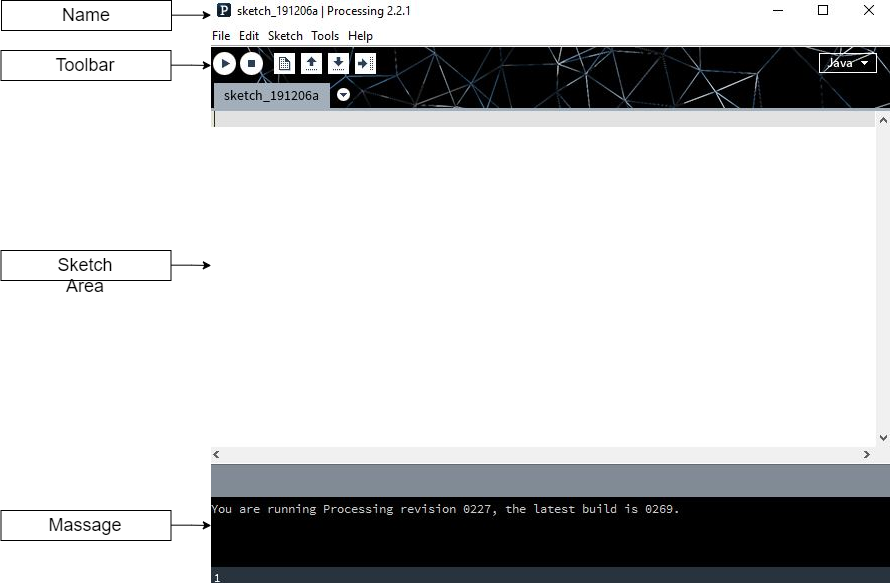
\includegraphics[width=12cm]{gambar/processing_view.png}
	\caption{Tampilan Processing IDE}
	\label{pic.processingide}
	\end{figure}


\subsection{\textit{Syntax} dalam Processing IDE }

\subsubsection{Mengatur Ukuran}
Ukuran sebuah objek pada processing IDE diatur menggunakan sebuah \textit{syntax} size(). Fungsi size() digunakan untuk menetapkan variabel global lebar dan tinggi dari suatu program. Ukuran untuk panjang dan tinggi tersebut menggunakan ukuran piksel. Lebar diwakili dengan variabel "\textit{width}" dan tinggi diwakili dengan variabel "\textit{height}". Untuk objek yang ukurannya tergantung pada layar, selalu gunakan variabel lebar dan tinggi, bukan angka. Ini mencegah masalah saat parameter fungsi size() diubah.


\subsubsection{Transformasi Bentuk dalam Processing IDE }
Transformasi pada Processing IDE digunakan untuk memindahkan, memutar atau, mengecilkan atau membesarkan suatu objek dan perpindahannya dapat diatur dengan parameter-parameter tertentu di dalam Processing IDE. Transformasi adalah dasar dari pemrograman Processing IDE. Tabel \ref{tbl.syntxtransformasi}  adalah adalah contoh penulisan \textit{syntax} dari Transformasi. 

\begin{table}[H]
	\centering
	\caption{ \textit{Syntax} Transformasi}
	\label{tbl.syntxtransformasi}
	\begin{tabular}{|c|l|l|}
		\hline
		No & \multicolumn{1}{c|}{\textit{Syntax}} & \multicolumn{1}{c|}{Keterangan}                                                            \\ \hline
		1  & Translate(x,y)                       & \begin{tabular}[c]{@{}l@{}}x = transisi kiri/kanan \\ y = transisi atas/bawah\end{tabular} \\ \hline
		2  & Rotate(angle)                        & angle=besar sudut rotasi(radian)                                                            \\ \hline
		3  & RotateX(angle)                       & angle=besar sudut rotasi(radian)                                                           \\ \hline
		4  & RotateY(angle)                       & angle=besar sudut rotasi(radian)                                                           \\ \hline
		5  & Rotatez(angle)                       & angle=besar sudut rotasi(radian)                                                           \\ \hline
		6  & Scale(S)                             & s = besar pengecilan pembesaran                                                         \\ \hline
	\end{tabular}
\end{table}
\subsubsection{Shape}
Shape adalah \textit{syntax} pada Processing IDE yang berfungsi untuk membuat berbagai macam bentuk, seperti persegi panjang, lingkaran, garis, dan bentuk lainnya yang dapat diatur ukurannya dengan parameter-parameter tertentu. Tabel \ref{tbl.syntxshape} merupakan contoh dari beberapa \textit{syntax} shape. 
\begin{table}[H]
	\centering
	\caption{\textit{Syntax} Shape}
	\label{tbl.syntxshape}
	\resizebox{14cm}{!}{%
	\begin{tabular}{|l|l|l|l|}
		\hline
		
		No & Sytax                          & Bentuk & Keterangan                                                                                                                                                                                    \\ \hline
		1  & ellipse(a,b,c,d)               &  	\centering 
\includegraphics[width=3cm]{gambar/bulat.png} 
& \begin{tabular}[c]{@{}l@{}}a = koordinatX \\ b = koordinatY \\ c= lebar diameter \\ d= tinggi diameter\end{tabular}                                                                           \\ \hline
		2  & arc(a,b,c,d,start,st op,moode) &  	
\includegraphics[width=3cm]{gambar/busur.png}      & \begin{tabular}[c]{@{}l@{}}a = koordinatX \\ b = koordinatY \\ c = lebar diameter \\ d = tinggi diameter \\ start = sudut mulai \\ stop = sudut akhir \\ mode = PIE, CHORD, OPEN\end{tabular} \\ \hline
		3  & line(x1,y1,x2,y2)              & 	
\includegraphics[width=3cm]{gambar/garis.png}       & \begin{tabular}[c]{@{}l@{}}x1 = koordinatX1 \\ y1 = koordinatY1 \\ x2 = koordinatX2 \\ y2 = koordinatY2\end{tabular}                                                                          \\ \hline
		4  & point(x,y)                     &     	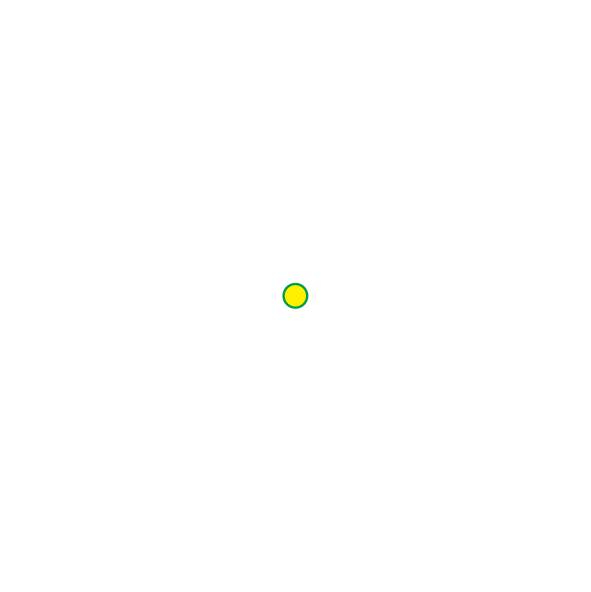
\includegraphics[width=0.5cm]{gambar/point.png}   & \begin{tabular}[c]{@{}l@{}}x = koordinatX \\ y = koordinatY\end{tabular}                                                                                                                      \\ \hline
		5  & rect(a,b,c,d,r)                &    	
\includegraphics[width=3cm]{gambar/kotak.png}    & \begin{tabular}[c]{@{}l@{}}a = koordinatX1 \\ b = koordinatY1 \\ c = koordinatX2 \\ d= koordinatY1\end{tabular}                                                                               \\ \hline
	\end{tabular}}
\end{table}

\subsubsection{Akses Koordinat Mouse }
Processing IDE mempunyai fungsi khusus yaitu dapat melacak posisi mouse baik secara vertical maupun horizontal. Namun, Processing IDE hanya dapat melacak posisi mouse saat sketch dijalankan saja. Nilai default mouseX dan mouseY adalah 0, jadi 0 akan dikembalikan sampai mouse bergerak di depan jendela sketsa. Setelah mouse bergerak menjauh dari jendela, mouseX akan terus melaporkan posisi terakhirnya. Tabel \ref{tbl.koordinatmouse}  merupakan contoh penulisan \textit{syntax} dari mouse. 
\begin{table}[H]
		\centering
	\caption{\textit{Syntax} Koordinat Mouse}
	\label{tbl.koordinatmouse}
	\begin{tabular}{|c|l|l|}
		\hline
		No & \multicolumn{1}{c|}{\textit{Syntax}} & \multicolumn{1}{c|}{Keterangan}                                                                                                 \\ \hline
		1  & mouseX                               & \begin{tabular}[c]{@{}l@{}}Variabel sistem X memiliki nilai dari \\ koordinat horizontal mouse secara real time\end{tabular}    \\ \hline
		2  & mouseY                               & \begin{tabular}[c]{@{}l@{}}Variabel sistem Y memiliki nilai dari koordinat \\ horizontal mouse secara real time.\end{tabular}   \\ \hline
		3  & mouseButton()                        & \begin{tabular}[c]{@{}l@{}}Bila tombol mouse ditekan, nilai variable sistem \\ disetel ke LEFT,RIGHT, atau CENTER.\end{tabular} \\ \hline
		4  & mouseClicked()                       & \begin{tabular}[c]{@{}l@{}}Dipanggil setelah tombol mouse ditekan \\ dan kemudian dilepaskan.\end{tabular}                      \\ \hline
		5  & mouseDragged()                       & Dipanggil setelah tombol mouse bergerak saat ditekan.                                                                           \\ \hline
	\end{tabular}
\end{table}

\subsubsection{ \textit{Compile Sketch} }
Program pada Processing IDE dinamakan \textit{sketch}. Tujuan diberi nama \textit{sketch} adalah untuk membuat pemrograman bergaya Java ini terasa lebih seperti \textit{scripting}, dan mengadopsi proses \textit{scripting} untuk menulis kode dengan cepat. \textit{Sketch} disimpan dalam bentuk \textit{Sketchbook}. Gambar \ref{pic.toolbarsketch} merupakan \textit{toolbar} dari \textit{sketch.}

	\begin{figure}[H]
	\centering
	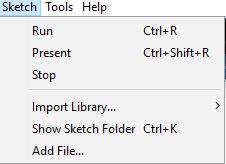
\includegraphics[width=5cm]{gambar/compile.jpg}
	\caption{\textit{Toolbar Sketch}}
	\label{pic.toolbarsketch}
\end{figure}

\subsection{ \textit{Library} untuk Processing IDE }
\subsubsection{ Memuat Huruf (\textit{Font}) pada Processing IDE }
Pfont adalah \textit{class} yang digunakan untuk penggunaan \textit{font} pada Processing IDE. Untuk membuat \textit{font} yang akan digunakan dengan Processing IDE, diawali dengan memilih "\textit{Create Font ...}" dari menu \textit{Tools}. Ini akan membuat \textit{font} dalam format Processing IDE yang membutuhkan dan juga menambahkannya ke direktori data sketsa saat ini. Pengolahan menampilkan font menggunakan format font .vlw. Fungsi loadFont() digunakan untuk membuat \textit{font} baru dan textFont () digunakan agar \textit{font} baru yang telah dibuat tersebut aktif. \textit{Syntax} list() berfungsi untuk membuat daftar \textit{font} yang terinstal di komputer, yang merupakan informasi yang berguna untuk digunakan dengan fungsi createFont() untuk mengubah \textit{font} secara dinamis menjadi format yang bisa digunakan di Processing IDE. 


\subsubsection{ Memuat ControlP5 pada Processing IDE }
ControlP5 adalah \textit{library} yang berfungsi sebagai pengontrol untuk membuat antarmuka dengan \textit{user}, ControlP5 berupa grafis di dalam \textit{sketch} Processing IDE yang meliputi \textit{Slider}, \textit{Button}, \textit{Toggles}, \textit{Knobs}, \textit{Radiobutton}, dan dapat dengan mudah ditambahkan ke \textit{sketch} pengolahan. ControlP5 ditulis oleh Andreas Schlegel untuk pemrograman Processing IDE. \textit{Library} ControlP5 bisa diunduh di laman https://github.com/sojamo/controlp5, atau unduh di \textit{library} Processing IDE secara langsung. Gambar \ref{pic.controlp5} merupakan beberapa contoh gambaran dari ControlP5.
	\begin{figure}[H]
	\centering
	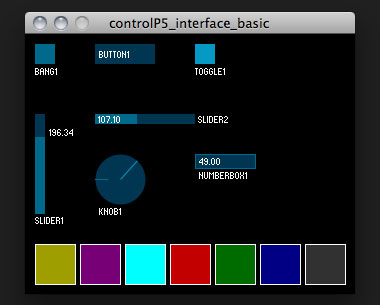
\includegraphics[width=8cm]{gambar/controlp5.jpg}
	\caption{ControlP5}
	\label{pic.controlp5}
\end{figure}
Setiap \textit{tools} yang ada pada ControlP5 memiliki fungsi yang berbeda-beda sesuai dengan kegunaannya. ControlP5 dapat dipakai atau saling dikombinasikan agar memudahkan dan memaksimalkan dari GUI yang telah dibuat. ControlP5 nantinya akan bekerja sesuai dengan program yang sudah dimasukkan. Pada Tabel \ref{tbl.toolscontrolp5} merupakan beberapa fungsi dari \textit{tools} yang ada pada ControlP5.
\begin{table}[H]
		\centering
	\caption{Fungsi \textit{Tools} ControlP5}
	\label{tbl.toolscontrolp5}
	\resizebox{14cm}{!}{%
	\begin{tabular}{|c|l|l|l|}
		\hline
		1 & Bang      & Memicu sebuah tindakan ketika ditekan                                                                               & controlP5.addBang("bang1");           \\ \hline
		2 & Button    & Memicu sebuah tindakan ketika sudah dilepas                                                                         & controlP5.addButton("button1");       \\ \hline
		3 & Toggle    & \begin{tabular}[c]{@{}l@{}}Memiliki dua status. \\ TRUE meiliki nilai 1 dan FALSE memiliki nilai 0\end{tabular}     & controlP5.addToggle("toggle1")        \\ \hline
		4 & Slider    & \begin{tabular}[c]{@{}l@{}}Mengatur nilai dengan cara menggeser \\ secara horisontal maupun vertikal\end{tabular}   & controlP5.addSlider("slider2");       \\ \hline
		5 & Knob      & Mengatur sebuah nilai dengan tombol putaran 360°                                                                    & controlP5.addKnob("knob1");           \\ \hline
		6 & NumberBox & \begin{tabular}[c]{@{}l@{}}Kotak yang menampilkan angka dan \\ dapat diubah dengan klik di dalam kotak\end{tabular} & controlP5.addNumberbox("numberbox1"); \\ \hline
	\end{tabular}}
\end{table}

